\documentclass[12pt,a4paper]{article}
\usepackage[latin1]{inputenc}
\usepackage[english]{babel}
\usepackage{amsmath}
\usepackage{amsfonts}
\usepackage{amssymb}
\usepackage{makeidx}
\usepackage{lmodern}
\usepackage{fourier}
\usepackage{listings}
\usepackage{xcolor} 

\usepackage{calc}
\usepackage{flowchart} % also loads tikz
\usetikzlibrary{arrows}


%
\definecolor{hellgelb}{rgb}{1,1,0.8}
\definecolor{colKeys}{rgb}{0,0,1}
\definecolor{colIdentifier}{rgb}{0,0,0}
\definecolor{colComments}{rgb}{1,0,0}
\definecolor{colString}{rgb}{0,0.5,0}

\lstset{%
    float=hbp,%
    basicstyle=\ttfamily\small, %
    identifierstyle=\color{colIdentifier}, %
    keywordstyle=\color{colKeys}, %
    stringstyle=\color{colString}, %
    commentstyle=\color{colComments}, %
    columns=flexible, %
    tabsize=2, %
    frame=single, %
    extendedchars=true, %
    showspaces=false, %
    showstringspaces=false, %
    numbers=left, %
    numberstyle=\tiny, %
    breaklines=true, %
    backgroundcolor=\color{hellgelb}, %
    breakautoindent=true, %
    captionpos=b%
}

\usepackage{float} 
\newfloat{Listing}{hbp}{lis}[section]

\newcommand{\MueLu}{MueLu}
\newcommand{\Xpetra}{Xpetra}

\author{Tobias Wiesner}
\begin{document}
\section{Tutorial 1}
\subsection{Welcome}
Welcome to \MueLu, the next generation multigrid package in Trilinos. This tutorial demonstrates how to generate a multigrid hierarchy for a 1D Laplace equation using MueLu.

The outline of this very first tutorial is as follows. In the next section we present a small test program for a 1D Laplace equation. We use this test program with different sets of multigrid parameters and show the basics of the xml input deck of \MueLu. In the last section we give an overview of the factories involved in generating smoothed aggregation transfer operators.

\subsection{Test program}
A rather general test program can be found in \texttt{tutorial1.cpp}. The purpose of this test program is to provide a framework to be able to test different multigrid parameters. The program first creates a 1D Laplace test problem, then builds a multigrid hierarchy using some parameters from user given xml parameter files and finally solves the problem using the multigrid solver or using a Krylov subspace method with the generated multigrid method as preconditioner. In the following paragraphs we shortly explain the different parts of the test program and give some common remarks on how to use \MueLu. 

\paragraph{Input variables}
The minimum input that is needed to generate a multigrid hierarchy is a fine level matrix $A$ and the corresponding near null space (or near kernel) of the fine level matrix $A$. \MueLu~is completely based on \Xpetra, a thin wrapper for the linear algebra packages Epetra and Tpetra in Trilinos. That is, the input information for \MueLu~has to be an \Xpetra~matrix object for the fine level matrix $A$ as well as an \Xpetra~multi vector for the null space.

Listing \ref{listing:galeri1dlaplace} gives an example how to generate a 1D Laplace example using the Galeri package. First, a global map has to be generated using the given communicator object. When creating the map, the user can choose either Epetra or Tpetra as underlying linear algebra framework. Then, the system matrix $A$ is generated using the global map. For a 1D Laplace example a constant vector is a good approximation for the near null space.
\begin{Listing} 
\begin{center} 
\begin{lstlisting}[language=C++,label=listing:galeri1dlaplace]
RCP<Matrix>      A;
RCP<MultiVector> nullspace;

RCP<const Teuchos::Comm<int> > comm = Teuchos::DefaultComm<int>::getComm();

Teuchos::ParameterList galeriList;
galeriList.set("nx", 100);
    
// generate map
RCP<const Map> map = Galeri::Xpetra::CreateMap<LO, GO, Node> (Xpetra::UseEpetra, "Cartesian1D", comm, galeriList);

// generate 1D Laplace matrix
RCP<Galeri::Xpetra::Problem<Map,CrsMatrixWrap,MultiVector> > Pr =
        Galeri::Xpetra::BuildProblem<SC,LO,GO,Map,CrsMatrixWrap,MultiVector>("Laplace1D", map, galeriList);
A = Pr->BuildMatrix();

// generate 1D null space vector
nullspace = MultiVectorFactory::Build(map, 1);
nullspace->putScalar(Teuchos::ScalarTraits<SC>::one());
\end{lstlisting}
\caption{Generate 1D Laplace problem using Galeri::Xpetra.} 
\label{listing:galeri1dlaplace}
\end{center}
\end{Listing}

In listing \ref{listing:epetra2xpetra} one can find how to transform given Epetra objects for the system matrix, right hand side as well as (near) null space to \Xpetra.
\begin{Listing} 
\begin{center} 
\begin{lstlisting}[language=C++,label=listing:epetra2xpetra]
RCP<Matrix>      A;
RCP<MultiVector> nullspace;

RCP<Epetra_CrsMatrix> epA = ... // System matrix (Epetra)
RCP<Epetra_Vector> epv = ...    // RHS vector (Epetra)
RCP<Epetra_MultiVector> epNS = ... // null space (multi) vector

// Epetra_CrsMatrix -> Xpetra::Matrix
RCP<CrsMatrix> exA = Teuchos::rcp(new Xpetra::EpetraCrsMatrix(epA));
RCP<CrsMatrixWrap> crsOp = Teuchos::rcp(new CrsMatrixWrap(exA));
A = Teuchos::rcp_dynamic_cast<Matrix>(crsOp);
A->SetFixedBlockSize(1); // assuming 1 DOF per node

// Epetra_Vector -> Xpetra::Vector
RCP<Vector> xRhs = Teuchos::rcp(new Xpetra::EpetraVector(epv));
nullspace = Teuchos::rcp(new Xpetra::EpetraMultiVector(epNS));

// Epetra_Map -> Xpetra::Map
const RCP< const Map> map = Xpetra::toXpetra(epA->RowMap());
\end{lstlisting}
\caption{Generate Xpetra objects from Epetra objects.} 
\label{listing:epetra2xpetra}
\end{center}
\end{Listing}

\paragraph{Multigrid setup}
Assuming the fine level matrix $A$ and the corresponding fine level near null space to be available we can generate the multigrid hiearchy. Following the code in listing \ref{listing:mueluhierarchy} we first create a \verb|ParameterListInterpreter| object which interprets some input parameters from the xml file "tutorial1.xml". A description of the xml parameter file follows in the next subsection.
Once a \verb|Hierarchy| object has been created it is filled with the available fine level information. Finally the \verb|SetupHierarchy| function is called which actually generates the multigrid hierarchy.
\begin{Listing} 
\begin{center} 
\begin{lstlisting}[language=C++,label=listing:epetra2xpetra]
ParameterListInterpreter mueLuFactory("tutorial1.xml", *comm);
RCP<Hierarchy> H = mueLuFactory.CreateHierarchy();

H->GetLevel(0)->Set("A",           A);
H->GetLevel(0)->Set("Nullspace",   nullspace);
mueLuFactory.SetupHierarchy(*H);
\end{lstlisting}
\caption{Build multigrid hierarchy} 
\label{listing:mueluhierarchy}
\end{center}
\end{Listing}

\paragraph{Multigrid as solver}
After the multigrid hierarchy object has been built and filled we can use it to solve a linear system.
Listing \ref{amgassolver} demonstrates how to do $25$ sweeps with the previously generated multigrid method. Therein \verb|X| is a given vector with an initial guess for the solution. Finally it stores the solution vector. Vector \verb|B| is the right hand side vector.
\begin{Listing} 
\begin{center} 
\begin{lstlisting}[language=C++,label=listing:AmgAsSolver]
H->IsPreconditioner(false);
H->Iterate(*B, 25, *X);
\end{lstlisting}
\caption{Use AMG as solver.} 
\label{listing:amgassolver}
\end{center}
\end{Listing}

\paragraph{Multigrid as preconditioner}
Another option is to use the \MueLu hierarchy as preconditioner within a Krylov subspace solver such as CG or GMRES. In listing \ref{listing:amgaspreconditioner} an example is shown how to use the \verb|Hierarchy| as a preconditioner for a CG method from the Belos package.
Again \verb|X| is the solution vector with a given initial guess. Vector \verb|B| is the right hand side vector.
\begin{Listing} 
\begin{center} 
\begin{lstlisting}[language=C++,label=listing:AmgAsPreconditioner]
// Operator and Multivector type that will be used with Belos
typedef MultiVector          MV;
typedef Belos::OperatorT<MV> OP;

H->IsPreconditioner(true);

// Define Operator and Preconditioner
RCP<OP> belosOp   = rcp(new Belos::XpetraOp<SC, LO, GO, NO, LMO>(A)); // Turns a Xpetra::Matrix object into a Belos operator
RCP<OP> belosPrec = rcp(new Belos::MueLuOp<SC, LO, GO, NO, LMO>(H));  // Turns a MueLu::Hierarchy object into a Belos operator

// Construct a Belos LinearProblem object
RCP< Belos::LinearProblem<SC, MV, OP> > belosProblem = rcp(new Belos::LinearProblem<SC, MV, OP>(belosOp, X, B));
belosProblem->setLeftPrec(belosPrec);
belosProblem->setProblem();

// Belos parameter list
ParameterList belosList;
belosList.set("Maximum Iterations",    200); 
belosList.set("Convergence Tolerance", 1e-5);   
belosList.set("Verbosity",             Belos::Errors );
belosList.set("Output Frequency",      1);
belosList.set("Output Style",          Belos::Brief);

// Create an iterative solver manager
RCP< Belos::SolverManager<SC, MV, OP> > solver;
solver = rcp(new Belos::BlockCGSolMgr<SC, MV, OP>(belosProblem, rcp(&belosList, false)));

// Perform solve
Belos::ReturnType ret = Belos::Unconverged;
ret = solver->solve();
cout << "Number of iterations: " << solver->getNumIters() << endl;
\end{lstlisting}
\caption{Use AMG as preconditioner within Belos.} 
\label{listing:amgaspreconditioner}
\end{center}
\end{Listing}

\subsection{Tutorial 1a: Basic XML parameters}
The setup routine for the multigrid hiearchy is controled by the xml file used as input for the \verb|ParameterListInterpreter| object.

Listing \ref{listing:minimalXML} gives a minimal example for a \MueLu XML input file. The most important part is the \textit{Hierarchy} section where basic parameters for the multigrid hierarchy are defined, such as the maximum allowed number of multigrid levels, the maximum allowed size of the coarse grid problem before coarsening stops or the verbosity level for screen output. In listing \ref{listing:minimalXML} the \textit{Factories} section is empty, i.e. default settings are assumed for building the multigrid hierarchy.
Per default a smoothed aggregation algebraic multigrid method is used, that is designed for symmetric positive definite problems. A standard Galerkin product operator is used to build the coarse level matrices by computing the $RAP$ product (without load rebalancing). The restriction operator is the transposed of the smoothed prolongation operator that is generated using information from a coupled aggregation strategy. The coupled aggregation strategy allows aggregates which overlap processor boundaries. As multigrid level smoother one sweep with an undamped symmetric Gauss Seidel method is applied. On the coarsest level we use a direct solver.
Even if the default settings are a good choice for most symmetric problems it is important to adapt the parameters to the underlaying problem. In the next sections we demonstrate how to change some parameters using the XML input deck.
\begin{Listing} 
\begin{center} 
\begin{lstlisting}[language=XML,label=listing:minimalXML]
<ParameterList name="MueLu">

  <!-- Configuration of the Xpetra operator (fine level) -->
  <ParameterList name="Matrix">
    <Parameter name="PDE equations" type="int" value="1"/> <!-- Number of PDE equations at each grid node.-->
  </ParameterList>

  <!-- Factory collection -->
  <ParameterList name="Factories">

  </ParameterList>

  <!-- Definition of the multigrid preconditioner -->
  <ParameterList name="Hierarchy">

    <Parameter name="numDesiredLevel" type="int"      value="10"/> <!-- Max number of levels -->
    <Parameter name="maxCoarseSize" type="int"      value="1000"/> <!-- Min number of rows on coarsest level -->
    <Parameter name="verbosity" type="string"   value="High"/> <!--None, Low, Medium, High, Extreme -->
  </ParameterList>
</ParameterList>

\end{lstlisting}
\caption{Structure of XML input file for \MueLu} 
\label{listing:minimalXML}
\end{center}
\end{Listing}

\subsection{Tutorial 1b: Level smoothers}
\begin{Listing} 
\begin{center} 
\begin{lstlisting}[language=XML,label=listing:chebyXML]
<ParameterList name="MueLu">

  <ParameterList name="Factories">

    <ParameterList name="myChebyshev">
      <Parameter name="factory" type="string" value="TrilinosSmoother"/>
      <Parameter name="type" type="string" value="CHEBYSHEV"/>

      <ParameterList name="ParameterList">
        <Parameter name="chebyshev: degree" type="int" value="1"/>
        <Parameter name="chebyshev: ratio eigenvalue" type="double" value="20"/>
        <Parameter name="chebyshev: min eigenvalue" type="double" value="1.0"/>
        <Parameter name="chebyshev: zero starting solution" type="bool" value="true"/>
      </ParameterList>
    </ParameterList>

  </ParameterList>

  <ParameterList name="Hierarchy">
    <Parameter name="numDesiredLevel" type="int"      value="10"/> 
    <Parameter name="maxCoarseSize" type="int"      value="10"/> 
    <Parameter name="verbosity" type="string"   value="Low"/>
    <ParameterList name="AllButCoarsestLevel">
      <Parameter name="startLevel" type="int"      value="0"/>
      <Parameter name="Smoother" type="string"   value="myChebyshev"/>
    </ParameterList>
    <ParameterList name="CoarsestLevel">
      <Parameter name="CoarseSolver" type="string"   value="DirectSolver"/>
    </ParameterList>
  </ParameterList>
</ParameterList>
\end{lstlisting}
\caption{Structure of XML input file for \MueLu with Chebyshev level smoother} 
\label{listing:chebyXML}
\end{center}
\end{Listing}

In listing \ref{listing:chebyXML} we replace the default symmetric Gauss Seidel sweeps by some Chebyshev polynomial smoother. In the \textit{Factories} section of the XML input file we first define a new section for our new Chebyshev smoother. We name it "myChebyshev", but any other name would also be ok.
The "myChebyshev" smoother is a \textit{TrilinosSmoother} of type \textit{CHEBYSHEV}. The \textit{TrilinosSmoother} class provides all iterative and polynomial smoothers such as Jacobi, Gauss Seidel and variants and Chebyshev. The internal parameter list within the "myChebyshev" section is used to define the smoother specific parameters, e.g. the number of sweeps and damping parameters or the polynomial degree. Most of the parameters are self-explaining and can be found in the documentation.

Once we have defined our new smoother factory we have to use it within our multigrid hierarchy. Here we add a new subsection to the \textit{Hierarchy} section with the fixed name "AllButCoarsestLevel". Therein we define the "Smoother" to be of type "myChebyshev", where the name must be exactly the same of the factory that we've declared before.

The subsection "CoarsestLevel" can be used to define some special factories for the coarsest level. In our example we explicitely define the "CoarseSolver" variable to be a direct solver.

\subsection{Tutorial 1c: More level smoothers}
\begin{Listing} 
\begin{center} 
\begin{lstlisting}[language=XML,label=listing:sgsXML]
<ParameterList name="MueLu">

  <ParameterList name="Factories">
    <ParameterList name="mySymGaussSeidel">
      <Parameter name="factory"                             type="string" value="TrilinosSmoother"/>
      <Parameter name="type"                                type="string" value="RELAXATION"/>
      <ParameterList name="ParameterList">
        <Parameter name="relaxation: type"                  type="string" value="Symmetric Gauss-Seidel"/>
        <Parameter name="relaxation: sweeps"                type="int"    value="2"/>
        <Parameter name="relaxation: damping factor"        type="double" value="1"/>
      </ParameterList>
    </ParameterList>

  </ParameterList>

  <ParameterList name="Hierarchy">
    <Parameter name="numDesiredLevel" type="int" value="10"/> 
    <Parameter name="maxCoarseSize" type="int" value="10"/> 
    <ParameterList name="AllButCoarsestLevel">
      <Parameter name="startLevel" type="int" value="0"/>
      <Parameter name="Smoother" type="string" value="mySymGaussSeidel"/>
    </ParameterList>
    <ParameterList name="CoarsestLevel">
      <Parameter name="CoarseSolver" type="string"   value="mySymGaussSeidel"/>
    </ParameterList>

  </ParameterList>
</ParameterList>

\end{lstlisting}
\caption{Structure of XML input file for \MueLu~ with symmetric GaussSeidel level smoothers} 
\label{listing:sgsXML}
\end{center}
\end{Listing}

Listing \ref{listing:sgsXML} is very similar to listing \ref{listing:chebyXML}. The only difference is, that now we use 2 sweeps with undamped symmetric Gauss Seidel as level smoother on all multigrid levels. We also replaced the direct solver on the coarsest level with the symmetric Gauss Seidel smoother.


\subsection{Tutorial 1d: Plain aggregation}
\begin{Listing} 
\begin{center} 
\begin{lstlisting}[language=XML,label=listing:plainAggregationXML]
<ParameterList name="MueLu">
  <ParameterList name="Factories">
    <ParameterList name="UncoupledAggregationFact">
      <Parameter name="factory" type="string" value="UncoupledAggregationFactory"/>
      <Parameter name="Ordering" type="string" value="Natural"/>
      <Parameter name="MaxNeighAlreadySelected" type="int" value="0"/>
      <Parameter name="MinNodesPerAggregate" type="int" value="2"/>
    </ParameterList>  
    <ParameterList name="myTentativePFact">
      <Parameter name="factory" type="string" value="TentativePFactory"/>
    </ParameterList>
    <ParameterList name="myRestrictorFact">
      <Parameter name="factory" type="string" value="TransPFactory"/>
      <Parameter name="P" type="string" value="myTentativePFact"/>
    </ParameterList>
  </ParameterList>

  <ParameterList name="Hierarchy">

    <Parameter name="numDesiredLevel" type="int"      value="10"/> 
    <Parameter name="maxCoarseSize" type="int"      value="10"/>
    <ParameterList name="AllButCoarsestLevel">
      <Parameter name="startLevel" type="int"      value="0"/>
      <Parameter name="Aggregates" type="string"   value="UncoupledAggregationFact"/>
      <Parameter name="Nullspace" type="string"   value="myTentativePFact"/>
      <Parameter name="P" type="string"   value="myTentativePFact"/>
      <Parameter name="R" type="string"   value="myRestrictorFact"/>
    </ParameterList>
  </ParameterList>
</ParameterList>
\end{lstlisting}
\caption{Structure of XML input file for \MueLu~ with plain aggregation transfer operators} 
\label{listing:plainAggregationXML}
\end{center}
\end{Listing}

In listing \ref{listing:plainAggregationXML} we demonstrate how to use non-smoothed transfer operators and a user-defined aggregation strategy. Again we define a "myTentativePFact" object of type "TentativePFactory" in the \textit{Factories} section. The restriction operator just shall be built as $R=P^T$. Therefore we add a "myRestrictorFact" of type "TransPFactory" and declare to use "myTentativePFact" as input variable "P" for "myRestrictorFact". This way we build the transpose of the tentative prolongation operator generated by "myTentativePFact" and store it as restriction operator (generated by "myRestrictorFact").

Furthermore, we want to be somewhat more specific about the aggregates. We define a "UncoupledAggregationFact" object to be of type "UncoupledAggregationFactory", where we can define some more aggregation parameters such as the minimum size of nodes per aggregate. We no want to use our "UncoupledAggregationFact" object to generate the aggregates that are used within our "myTentativePFact" prolongation operator factory. In general we have several options to do that. We could either add an additional parameter "Aggregates" in our "myTentativePFact" object and declare the aggregates built with the "UncoupdledAggregationFact" object to be input of the tentative prolongation factory (similar to how we did it for variable "P" in "myRestrictorFact"). The alternative is to declare our "UncoupledAggregationFact" to be our default factory for the variable "Aggregates", as it is done in listing \ref{listing:plainAggregationXML} by adding a parameter entry for the variable "Aggregates" in the "AllButCoarsestLevel" section.

A closer look to the "AllButCoarsestLevel" parameter section reveals, that beside of the entries for the variables "P", "R" and "Aggregates" we also have an entry for the variable "Nullspace" which points to the "myTentativePFactory". This is important. Some factories (e.g. the TentativePFactory) produce different variables (namely for TentativePFactory it is "P" for the non-smoothed transfer operator and "Nullspace" for the coarse level null space vector). If a factory generates different variables we have to make sure that we use the same factory for all these variables. Otherwise the factory manager would create a new instance for the default factory of the variable, which could either mean that some data is calculated twice or the program is just crashing, since the data is not consistent any more.

\subsection{General workflow of multigrid setup}

\begin{figure}
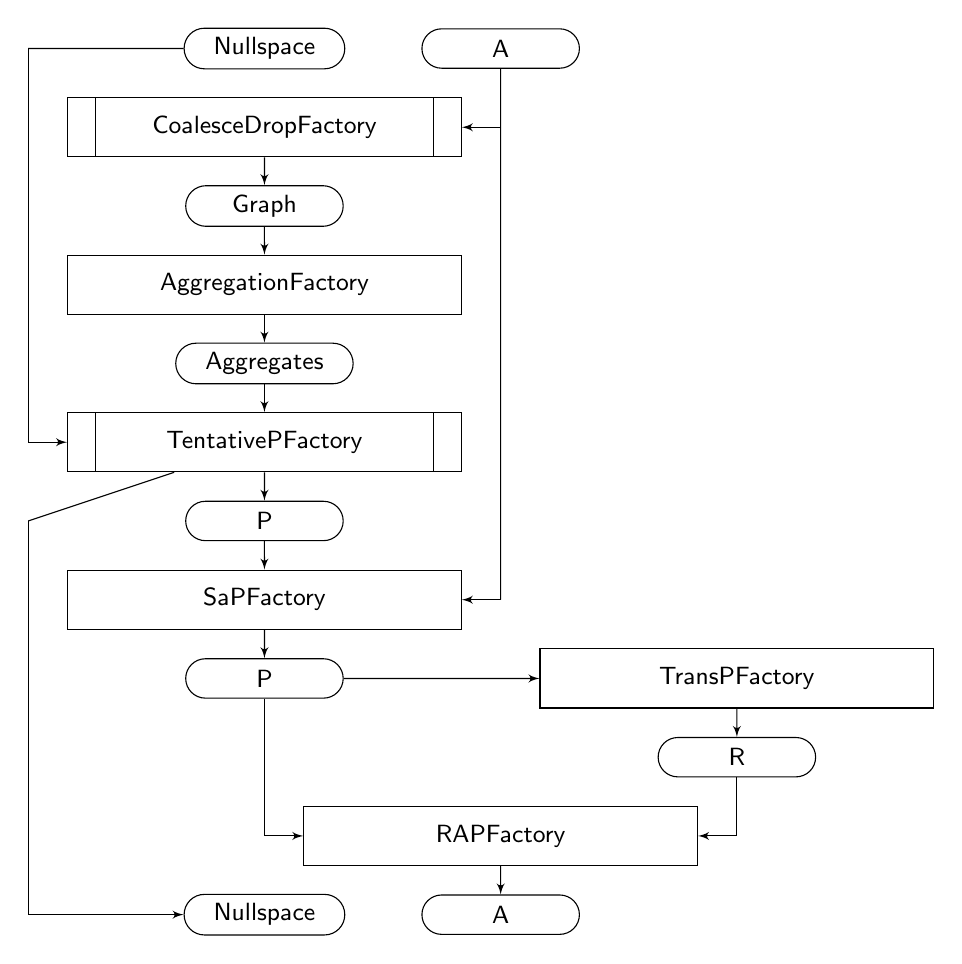
\begin{tikzpicture}[>=latex',font={\sf \small}]
\def\datawidth{2cm}
\def\dataheight{0.5cm}
\def\factorywidth{5cm}
\def\factoryheight{0.75cm}

\node(A) at (3,1) [draw, terminal, minimum width=\datawidth, minimum height=\dataheight]{A};
\node(Nullspace) at (0,1) [draw, terminal, minimum width=\datawidth, minimum height=\dataheight]{Nullspace};
\coordinate (co1) at (-3,1);
\coordinate (co2) at (-3,-4);
\coordinate (co3) at (3,-6);
\coordinate (co4) at (-3,-5);
\node(CoalesceDropFactory) at (0,0) [draw, predproc, minimum width=\factorywidth, minimum height=\factoryheight]{CoalesceDropFactory};
\node(Graph) at (0,-1) [draw, terminal, minimum width=\datawidth, minimum height=\dataheight]{Graph};
\node(AggregationFactory) at (0,-2) [draw, process, minimum width=\factorywidth, minimum height=\factoryheight]{AggregationFactory};
\node(Aggregates) at (0,-3) [draw, terminal, minimum width=\datawidth, minimum height=\dataheight]{Aggregates};
\node(TentativePFactory) at (0,-4) [draw, predproc, minimum width=\factorywidth, minimum height=\factoryheight]{TentativePFactory};
\node(Ptent) at (0,-5) [draw, terminal, minimum width=\datawidth, minimum height=\dataheight]{P};
\node(SaPFactory) at (0,-6) [draw, process, minimum width=\factorywidth, minimum height=\factoryheight]{SaPFactory};
\node(P) at (0,-7) [draw, terminal, minimum width=\datawidth, minimum height=\dataheight]{P};
\node(TransPFactory) at (6,-7) [draw, process, minimum width=\factorywidth, minimum height=\factoryheight]{TransPFactory};
\node(R) at (6,-8) [draw, terminal, minimum width=\datawidth, minimum height=\dataheight]{R};
\node(RAPFactory) at (3,-9) [draw, process, minimum width=\factorywidth, minimum height=\factoryheight]{RAPFactory};
\node(A2) at (3,-10) [draw, terminal, minimum width=\datawidth, minimum height=\dataheight]{A};
\node(Nullspace2) at (0,-10) [draw, terminal, minimum width=\datawidth, minimum height=\dataheight]{Nullspace};
\draw[-] (Nullspace) -- (co1);
\draw[-] (co1) -- (co2);
\draw[->] (co2) -- (TentativePFactory);
\draw[->] (A) |- (CoalesceDropFactory);
\draw[->] (CoalesceDropFactory) -- (Graph);
\draw[->] (Graph) -- (AggregationFactory);
\draw[->] (AggregationFactory) -- (Aggregates);
\draw[->] (Aggregates) -- (TentativePFactory);
\draw[-]  (A) -- (co3);
\draw[->] (co3) -- (SaPFactory);
\draw[->] (TentativePFactory) -- (Ptent);
\draw[->] (Ptent) -- (SaPFactory);
\draw[->] (SaPFactory) -- (P);
\draw[->] (P) |- (RAPFactory);
\draw[->] (P) -- (TransPFactory);
\draw[->] (TransPFactory) -- (R);
\draw[->] (R) |- (RAPFactory);
\draw[-]  (TentativePFactory) -- (co4);
\draw[->] (co4) |- (Nullspace2);
\draw[->] (RAPFactory) -- (A2);
\end{tikzpicture}
\caption{General workflow for smoothed aggregation transfer operators and Galerkin product}
\label{fig:generalworkflow}
\end{figure}

In figure \ref{fig:generalworkflow} we show the process of generating smoothed aggregation transfer operators. We start with an approximation of the fine level null space and the fine level matrix $A$. 
First, the \textit{CoalesceDropFactory} builds the graph of the fine level matrix $A$. If requested by the user it is possible to apply some filtering strategy to the fine level matrix before the graph is built. The graph of matrix $A$ is then used to build aggregates. The fine level null space together with the aggregation information is needed to define the non-smoothed tentative prolongation operator with the \textit{TentativePFactory}. Be aware that there are some more connections between the \textit{CoalesceDropFactory} and the \textit{TentativePFactory}, which are not shown here for simplicity. In case of not just one DOF per node, the \textit{CoalesceDropFactory} makes use of a helper class \textit{AmalgamationFactory} which amalgamates the matrix for finding the amalgamated graph. The hidden \textit{AmalgamationFactory} provides some information which is used in the \textit{TentativePFactory} to reconstruct the unamalgamated transfer operators from the amalgamated aggregation information. More details follow in other tutorials with vector problems instead of scalar problems.

Note, that the \textit{TentativePFactory} both generates the non-smoothed tentative transfer operator as well as the coarse level null space. Once the tentative prolongation operator is built, it is smoothed using the \textit{SaPFactory}. The \textit{TransPFacotry} builds the restriction operator just by transposing the smoothed prolongation operator. Finally, the \textit{RAPFactory} builds the coarse level matrix $A$.

Alltogether, the algorithm ends with an approximation of the coarse level null space and a coarse matrix $A$.


\section{Tutorial 2}

% symmetric design of 2x2 blocked preconditioner with repartitioning
\scalebox{0.6}{
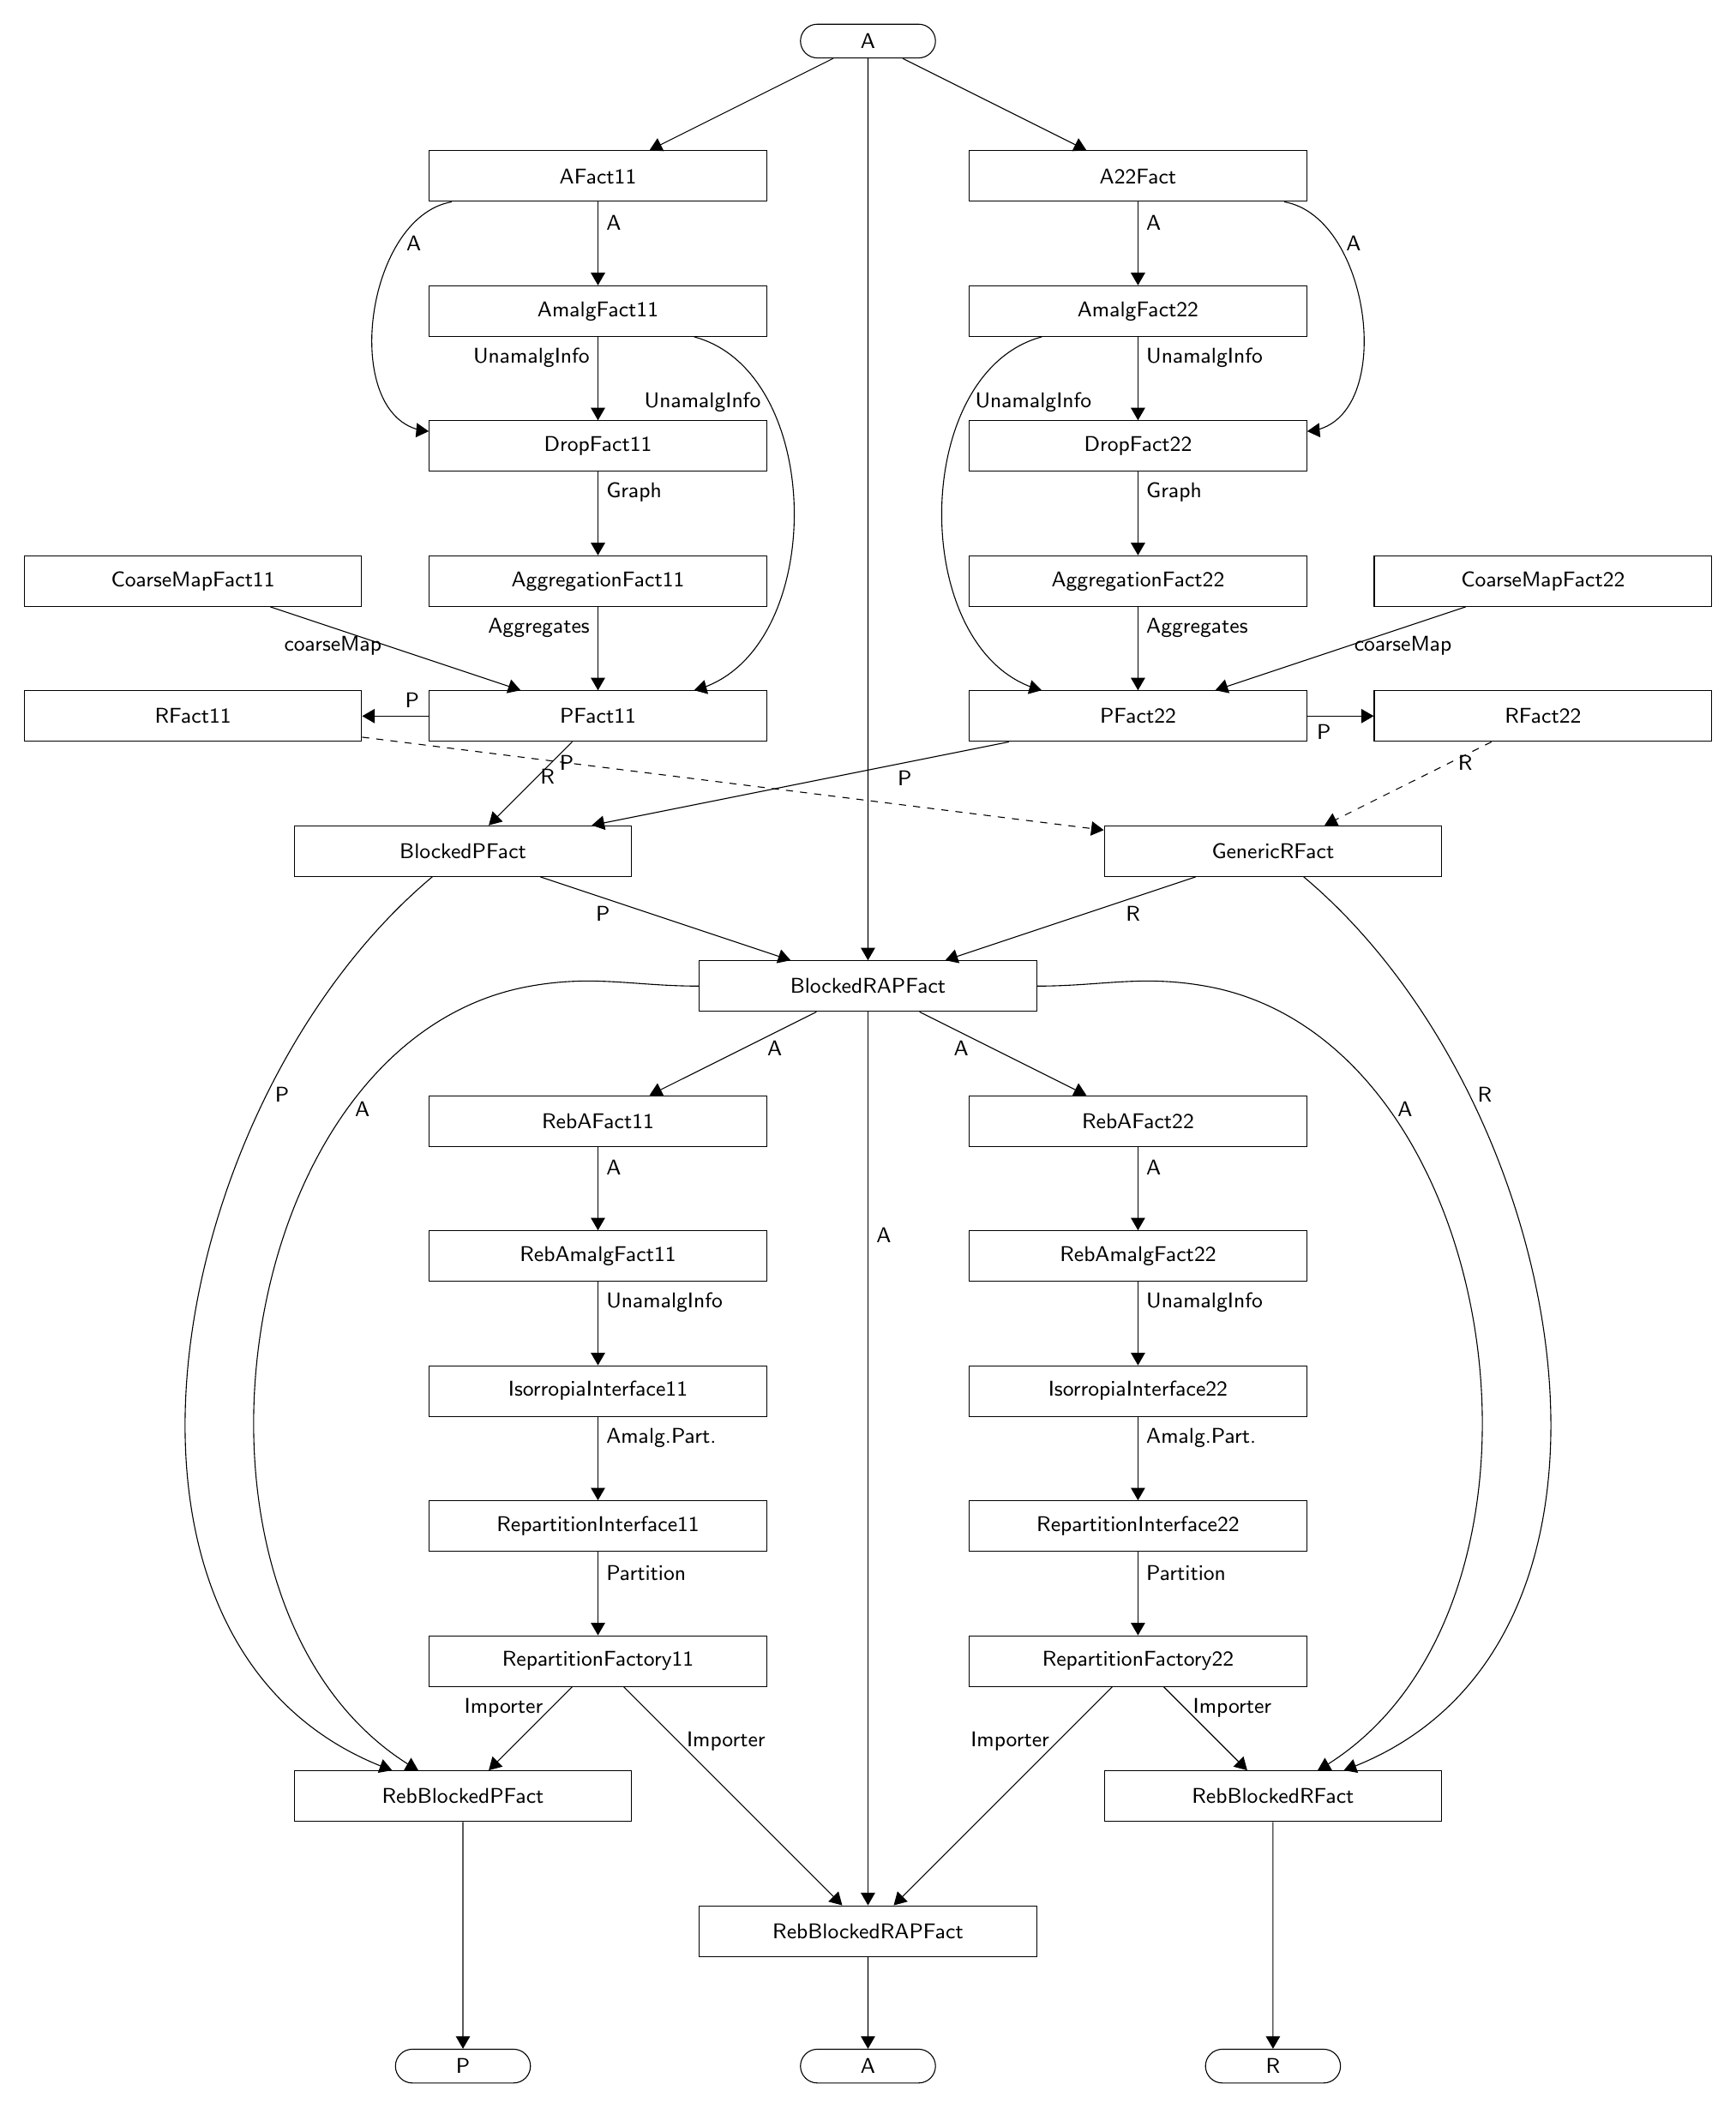
\begin{tikzpicture}[>=latex',font={\sf \small}, node distance=2cm]
\def\datawidth{2cm}
\def\dataheight{0.5cm}
\def\factorywidth{5cm}
\def\factoryheight{0.75cm}

%\draw[help lines] (-10,-10) grid (10,10);
\begin{scope}[>=triangle 60]
\node(A) at (1,10) [draw, terminal, minimum width=\datawidth, minimum height=\dataheight]{A};
\node(AFact11) at (-3,8) [draw, process, minimum width=\factorywidth, minimum height=\factoryheight]{AFact11};
\node [draw, process, minimum width=\factorywidth, minimum height=\factoryheight, below of=AFact11] (AmalgFact11) {AmalgFact11};
\node [draw, process, minimum width=\factorywidth, minimum height=\factoryheight, below of=AmalgFact11] (DropFact11) {DropFact11};
\node [draw, process, minimum width=\factorywidth, minimum height=\factoryheight, below of=DropFact11] (AggregationFact11) {AggregationFact11};
\node [draw, process, minimum width=\factorywidth, minimum height=\factoryheight, left of=AggregationFact11,node distance=6cm] (CoarseMapFact11) {CoarseMapFact11};
\node [draw, process, minimum width=\factorywidth, minimum height=\factoryheight, below of=AggregationFact11] (PFact11) {PFact11};
\node [draw, process, minimum width=\factorywidth, minimum height=\factoryheight, left of=PFact11,node distance=6cm] (RFact11) {RFact11};
\draw[->] (AFact11) -- node [near start, right] {A} (AmalgFact11);
\draw[->] (AFact11) to[out=190,in=175] node [near start, right] {A} (DropFact11);
\draw[->] (AmalgFact11) -- node [near start, left] {UnamalgInfo} (DropFact11);
\draw[->] (DropFact11) -- node [near start, right] {Graph} (AggregationFact11);
\draw[->] (AggregationFact11) -- node [near start, left] {Aggregates} (PFact11);
\draw[->] (PFact11) -- node [near start, above] {P} (RFact11);
\draw[->] (CoarseMapFact11) -- node [near start, below] {coarseMap} (PFact11);
\draw[->] (AmalgFact11) to[out=-15,in=15] node[near start, left] {UnamalgInfo} (PFact11);
\draw[->] (A) -- (AFact11);

\node [draw, process, minimum width=\factorywidth, minimum height=\factoryheight, right of=AFact11,node distance=8cm] (AFact22) {A22Fact};
\node [draw, process, minimum width=\factorywidth, minimum height=\factoryheight, below of=AFact22] (AmalgFact22) {AmalgFact22};
\node [draw, process, minimum width=\factorywidth, minimum height=\factoryheight, below of=AmalgFact22] (DropFact22) {DropFact22};
\node [draw, process, minimum width=\factorywidth, minimum height=\factoryheight, below of=DropFact22] (AggregationFact22) {AggregationFact22};
\node [draw, process, minimum width=\factorywidth, minimum height=\factoryheight, right of=AggregationFact22,node distance=6cm] (CoarseMapFact22) {CoarseMapFact22};
\node [draw, process, minimum width=\factorywidth, minimum height=\factoryheight, below of=AggregationFact22] (PFact22) {PFact22};
\node [draw, process, minimum width=\factorywidth, minimum height=\factoryheight, right of=PFact22,node distance=6cm] (RFact22) {RFact22};
\draw[->] (AFact22) -- node [near start, right] {A} (AmalgFact22);
\draw[->] (AFact22) to[out=-10,in=5] node [near start, right] {A} (DropFact22);
\draw[->] (AmalgFact22) -- node [near start, right] {UnamalgInfo} (DropFact22);
\draw[->] (DropFact22) -- node [near start, right] {Graph} (AggregationFact22);
\draw[->] (AggregationFact22) -- node [near start, right] {Aggregates} (PFact22);
\draw[->] (PFact22) -- node [near start, below] {P} (RFact22);
\draw[->] (CoarseMapFact22) -- node [near start, below] {coarseMap} (PFact22);
\draw[->] (AmalgFact22) to[out=195,in=165] node[near start, right] {UnamalgInfo} (PFact22);
\draw[->] (A) -- (AFact22);

\node (BlockedPFact) at (-5,-2) [draw, process, minimum width=\factorywidth, minimum height=\factoryheight]  {BlockedPFact};
\node [draw, process, minimum width=\factorywidth, minimum height=\factoryheight, right of=BlockedPFact,node distance=12cm] (GenericRFact) {GenericRFact};
\draw[->] (PFact11) -- node [near start, right] {P} (BlockedPFact);
\draw[->] (PFact22) -- node [near start, below] {P} (BlockedPFact);
\draw[->,dashed] (RFact11) -- node [near start, below] {R} (GenericRFact);
\draw[->,dashed] (RFact22) -- node [near start, right] {R} (GenericRFact);

\node (BlockedRAPFact) at (1,-4) [draw, process, minimum width=\factorywidth, minimum height=\factoryheight]  {BlockedRAPFact};
\draw[->] (BlockedPFact) -- node [near start, below] {P} (BlockedRAPFact);
\draw[->] (GenericRFact) -- node [near start, below] {R} (BlockedRAPFact);
\draw[->] (A) -- (BlockedRAPFact);

\node (RebAFact11) at (-3,-6) [draw, process, minimum width=\factorywidth, minimum height=\factoryheight]  {RebAFact11};
\node [draw, process, minimum width=\factorywidth, minimum height=\factoryheight, below of=RebAFact11] (RebAmalgFact11) {RebAmalgFact11};
\node [draw, process, minimum width=\factorywidth, minimum height=\factoryheight, below of=RebAmalgFact11] (IsorropiaInterface11) {IsorropiaInterface11};
\node [draw, process, minimum width=\factorywidth, minimum height=\factoryheight, below of=IsorropiaInterface11] (RepartitionInterface11){RepartitionInterface11};
\node [draw, process, minimum width=\factorywidth, minimum height=\factoryheight, below of=RepartitionInterface11] (RepartitionFactory11) {RepartitionFactory11};


\node (RebAFact22) at (5,-6) [draw, process, minimum width=\factorywidth, minimum height=\factoryheight]  {RebAFact22};
\node [draw, process, minimum width=\factorywidth, minimum height=\factoryheight, below of=RebAFact22] (RebAmalgFact22) {RebAmalgFact22};
\node [draw, process, minimum width=\factorywidth, minimum height=\factoryheight, below of=RebAmalgFact22] (IsorropiaInterface22) {IsorropiaInterface22};
\node [draw, process, minimum width=\factorywidth, minimum height=\factoryheight, below of=IsorropiaInterface22] (RepartitionInterface22){RepartitionInterface22};
\node [draw, process, minimum width=\factorywidth, minimum height=\factoryheight, below of=RepartitionInterface22] (RepartitionFactory22) {RepartitionFactory22};

\node (RebBlockedPFact) at (-5,-16) [draw, process, minimum width=\factorywidth, minimum height=\factoryheight]  {RebBlockedPFact};
\node [draw, process, minimum width=\factorywidth, minimum height=\factoryheight, right of=RebBlockedPFact,node distance=12cm] (RebBlockedRFact) {RebBlockedRFact};
\node (RebBlockedRAPFact) at (1,-18) [draw, process, minimum width=\factorywidth, minimum height=\factoryheight]  {RebBlockedRAPFact};
\coordinate [left of=BlockedRAPFact,node distance=5cm](coLeftOfBlockedRAPFact);
\coordinate [right of=BlockedRAPFact,node distance=5cm](coRightOfBlockedRAPFact);
\draw[->] (BlockedRAPFact) -- node [near start, right] {A} (RebBlockedRAPFact);
\draw[->] (BlockedRAPFact) to[out=180,in=10] (coLeftOfBlockedRAPFact) to[out=190,in=150] node[near start, right] {A} (RebBlockedPFact);
\draw[->] (BlockedPFact) to[out=220,in=160] node [near start, right] {P} (RebBlockedPFact);

\draw[->] (BlockedRAPFact) to[out=0,in=170] (coRightOfBlockedRAPFact) to[out=-10,in=30] node[near start, right] {A} (RebBlockedRFact);
\draw[->] (GenericRFact) to[out=-40,in=20] node [near start, right] {R} (RebBlockedRFact);

\draw[->] (BlockedRAPFact) -- node [near start, below] {A} (RebAFact11);
\draw[->] (RebAFact11) -- node [near start, right] {A} (RebAmalgFact11);
\draw[->] (RebAmalgFact11) -- node [near start, right] {UnamalgInfo} (IsorropiaInterface11);
\draw[->] (IsorropiaInterface11) -- node [near start, right] {Amalg.Part.} (RepartitionInterface11);
\draw[->] (RepartitionInterface11) -- node [near start, right] {Partition} (RepartitionFactory11);
\draw[->] (RepartitionFactory11) -- node [near start, left] {Importer} (RebBlockedPFact);
\draw[->] (RepartitionFactory11) -- node [near start, right] {Importer} (RebBlockedRAPFact);

\draw[->] (BlockedRAPFact) -- node [near start, below] {A} (RebAFact22);
\draw[->] (RebAFact22) -- node [near start, right] {A} (RebAmalgFact22);
\draw[->] (RebAmalgFact22) -- node [near start, right] {UnamalgInfo} (IsorropiaInterface22);
\draw[->] (IsorropiaInterface22) -- node [near start, right] {Amalg.Part.} (RepartitionInterface22);
\draw[->] (RepartitionInterface22) -- node [near start, right] {Partition} (RepartitionFactory22);
\draw[->] (RepartitionFactory22) -- node [near start, right] {Importer} (RebBlockedRFact);
\draw[->] (RepartitionFactory22) -- node [near start, left] {Importer} (RebBlockedRAPFact);

\node [draw, terminal, minimum width=\datawidth, minimum height=\dataheight, below of=RebBlockedRAPFact](Acoarse){A};
\node [draw, terminal, minimum width=\datawidth, minimum height=\dataheight, below of=RebBlockedPFact, node distance=4cm](Pcoarse){P};
\node [draw, terminal, minimum width=\datawidth, minimum height=\dataheight, below of=RebBlockedRFact, node distance=4cm](Rcoarse){R};
\draw[->] (RebBlockedRAPFact) -- (Acoarse);
\draw[->] (RebBlockedPFact) -- (Pcoarse);
\draw[->] (RebBlockedRFact) -- (Rcoarse);
\end{scope}
\end{tikzpicture}
} % end scalebox

% non-symmetric design of 2x2 block preconditioner with reusing aggregates of upper-left block
\scalebox{0.6}{
\begin{tikzpicture}[>=latex',font={\sf \small}, node distance=2cm]
\def\datawidth{2cm}
\def\dataheight{0.5cm}
\def\factorywidth{5cm}
\def\factoryheight{0.75cm}

%\draw[help lines] (-10,-10) grid (10,10);
\begin{scope}[>=triangle 60]
\node(A) at (1,10) [draw, terminal, minimum width=\datawidth, minimum height=\dataheight]{A};
\node(AFact11) at (-3,8) [draw, process, minimum width=\factorywidth, minimum height=\factoryheight]{AFact11};
\node [draw, process, minimum width=\factorywidth, minimum height=\factoryheight, below of=AFact11] (AmalgFact11) {AmalgFact11};
\node [draw, process, minimum width=\factorywidth, minimum height=\factoryheight, below of=AmalgFact11] (DropFact11) {DropFact11};
\node [draw, process, minimum width=\factorywidth, minimum height=\factoryheight, below of=DropFact11] (AggregationFact11) {AggregationFact11};
\node [draw, process, minimum width=\factorywidth, minimum height=\factoryheight, left of=AggregationFact11,node distance=6cm] (CoarseMapFact11) {CoarseMapFact11};
\node [draw, process, minimum width=\factorywidth, minimum height=\factoryheight, below of=AggregationFact11] (PFact11) {PFact11};
\node [draw, process, minimum width=\factorywidth, minimum height=\factoryheight, left of=PFact11,node distance=6cm] (RFact11) {RFact11};
\draw[->] (AFact11) -- node [near start, right] {A} (AmalgFact11);
\draw[->] (AFact11) to[out=190,in=175] node [near start, right] {A} (DropFact11);
\draw[->] (AmalgFact11) -- node [near start, left] {UnamalgInfo} (DropFact11);
\draw[->] (DropFact11) -- node [near start, right] {Graph} (AggregationFact11);
\draw[->] (AggregationFact11) -- node [near start, left] {Aggregates} (PFact11);
\draw[->] (PFact11) -- node [near start, above] {P} (RFact11);
\draw[->] (CoarseMapFact11) -- node [near start, below] {coarseMap} (PFact11);
\draw[->] (AmalgFact11) to[out=-15,in=15] node[near start, left] {UnamalgInfo} (PFact11);
\draw[->] (A) -- (AFact11);

\node [draw, process, minimum width=\factorywidth, minimum height=\factoryheight, right of=AFact11,node distance=8cm] (AFact22) {A22Fact};
\node [draw, process, minimum width=\factorywidth, minimum height=\factoryheight, below of=AFact22] (AmalgFact22) {AmalgFact22};
\node [draw, process, minimum width=\factorywidth, minimum height=\factoryheight, right of=AggregationFact22,node distance=6cm] (CoarseMapFact22) {CoarseMapFact22};
\node [draw, process, minimum width=\factorywidth, minimum height=\factoryheight, below of=AggregationFact22] (PFact22) {PFact22};
\node [draw, process, minimum width=\factorywidth, minimum height=\factoryheight, right of=PFact22,node distance=6cm] (RFact22) {RFact22};
\draw[->] (AFact22) -- node [near start, right] {A} (AmalgFact22);
\draw[->] (AmalgFact22) -- node [near start, right] {UnamalgInfo} (PFact22);
\draw[->] (PFact22) -- node [near start, below] {P} (RFact22);
\draw[->] (CoarseMapFact22) -- node [near start, below] {coarseMap} (PFact22);
\draw[->] (AggregationFact11) -- node [near end, above] {Aggregates} (PFact22);
\draw[->] (A) -- (AFact22);

\node (BlockedPFact) at (-5,-2) [draw, process, minimum width=\factorywidth, minimum height=\factoryheight]  {BlockedPFact};
\node [draw, process, minimum width=\factorywidth, minimum height=\factoryheight, right of=BlockedPFact,node distance=12cm] (GenericRFact) {GenericRFact};
\draw[->] (PFact11) -- node [near start, right] {P} (BlockedPFact);
\draw[->] (PFact22) -- node [near start, below] {P} (BlockedPFact);
\draw[->,dashed] (RFact11) -- node [near start, below] {R} (GenericRFact);
\draw[->,dashed] (RFact22) -- node [near start, right] {R} (GenericRFact);

\node (BlockedRAPFact) at (1,-4) [draw, process, minimum width=\factorywidth, minimum height=\factoryheight]  {BlockedRAPFact};
\draw[->] (BlockedPFact) -- node [near start, below] {P} (BlockedRAPFact);
\draw[->] (GenericRFact) -- node [near start, below] {R} (BlockedRAPFact);
\draw[->] (A) -- (BlockedRAPFact);

\node (RebAFact11) at (-3,-6) [draw, process, minimum width=\factorywidth, minimum height=\factoryheight]  {RebAFact11};
\node [draw, process, minimum width=\factorywidth, minimum height=\factoryheight, below of=RebAFact11] (RebAmalgFact11) {RebAmalgFact11};
\node [draw, process, minimum width=\factorywidth, minimum height=\factoryheight, below of=RebAmalgFact11] (IsorropiaInterface11) {IsorropiaInterface11};
\node [draw, process, minimum width=\factorywidth, minimum height=\factoryheight, below of=IsorropiaInterface11] (RepartitionInterface11){RepartitionInterface11};
\node [draw, process, minimum width=\factorywidth, minimum height=\factoryheight, below of=RepartitionInterface11] (RepartitionFactory11) {RepartitionFactory11};


\node (RebAFact22) at (5,-6) [draw, process, minimum width=\factorywidth, minimum height=\factoryheight]  {RebAFact22};
\node [draw, process, minimum width=\factorywidth, minimum height=\factoryheight, below of=RebAFact22] (RebAmalgFact22) {RebAmalgFact22};
\node [draw, process, minimum width=\factorywidth, minimum height=\factoryheight, below of=IsorropiaInterface22] (RepartitionInterface22){RepartitionInterface22};
\node [draw, process, minimum width=\factorywidth, minimum height=\factoryheight, below of=RepartitionInterface22] (RepartitionFactory22) {RepartitionFactory22};

\node (RebBlockedPFact) at (-5,-16) [draw, process, minimum width=\factorywidth, minimum height=\factoryheight]  {RebBlockedPFact};
\node [draw, process, minimum width=\factorywidth, minimum height=\factoryheight, right of=RebBlockedPFact,node distance=12cm] (RebBlockedRFact) {RebBlockedRFact};
\node (RebBlockedRAPFact) at (1,-18) [draw, process, minimum width=\factorywidth, minimum height=\factoryheight]  {RebBlockedRAPFact};
\coordinate [left of=BlockedRAPFact,node distance=5cm](coLeftOfBlockedRAPFact);
\coordinate [right of=BlockedRAPFact,node distance=5cm](coRightOfBlockedRAPFact);
\draw[->] (BlockedRAPFact) -- node [near start, right] {A} (RebBlockedRAPFact);
\draw[->] (BlockedRAPFact) to[out=180,in=10] (coLeftOfBlockedRAPFact) to[out=190,in=150] node[near start, right] {A} (RebBlockedPFact);
\draw[->] (BlockedPFact) to[out=220,in=160] node [near start, right] {P} (RebBlockedPFact);

\draw[->] (BlockedRAPFact) to[out=0,in=170] (coRightOfBlockedRAPFact) to[out=-10,in=30] node[near start, right] {A} (RebBlockedRFact);
\draw[->] (GenericRFact) to[out=-40,in=20] node [near start, right] {R} (RebBlockedRFact);

\draw[->] (BlockedRAPFact) -- node [near start, below] {A} (RebAFact11);
\draw[->] (RebAFact11) -- node [near start, right] {A} (RebAmalgFact11);
\draw[->] (RebAmalgFact11) -- node [near start, right] {UnamalgInfo} (IsorropiaInterface11);
\draw[->] (IsorropiaInterface11) -- node [near start, right] {Amalg.Part.} (RepartitionInterface11);
\draw[->] (RepartitionInterface11) -- node [near start, right] {Partition} (RepartitionFactory11);
\draw[->] (RepartitionFactory11) -- node [near start, left] {Importer} (RebBlockedPFact);
\draw[->] (RepartitionFactory11) -- node [near start, right] {Importer} (RebBlockedRAPFact);

\draw[->] (BlockedRAPFact) -- node [near start, below] {A} (RebAFact22);
\draw[->] (RebAFact22) -- node [near start, right] {A} (RebAmalgFact22);
\draw[->] (RebAmalgFact22) -- node [near start, right] {UnamalgInfo} (RepartitionInterface22);
\draw[->] (IsorropiaInterface11) -- node [near end, above] {Amalg.Part.} (RepartitionInterface22);
\draw[->] (RepartitionInterface22) -- node [near start, right] {Partition} (RepartitionFactory22);
\draw[->] (RepartitionFactory22) -- node [near start, right] {Importer} (RebBlockedRFact);
\draw[->] (RepartitionFactory22) -- node [near start, left] {Importer} (RebBlockedRAPFact);

\node [draw, terminal, minimum width=\datawidth, minimum height=\dataheight, below of=RebBlockedRAPFact](Acoarse){A};
\node [draw, terminal, minimum width=\datawidth, minimum height=\dataheight, below of=RebBlockedPFact, node distance=4cm](Pcoarse){P};
\node [draw, terminal, minimum width=\datawidth, minimum height=\dataheight, below of=RebBlockedRFact, node distance=4cm](Rcoarse){R};
\draw[->] (RebBlockedRAPFact) -- (Acoarse);
\draw[->] (RebBlockedPFact) -- (Pcoarse);
\draw[->] (RebBlockedRFact) -- (Rcoarse);
\end{scope}
\end{tikzpicture}
} % end scalebox
\end{document}